
% :::::: V - Experimental Evaluation ::::::::::::::::::
\section{Experimental Evaluation}
\label{Evaluation}

% Introductory paragraph
%%%%%%%%%%%%%%%%%%%%%%%%%%%%% .
In the empirical analysis, we evaluate the performance, accuracy and efficiency of the Convolutional Neural Network algorithm. In the following sections, we will discuss the experimental setup, how we did the experiments and the corresponding results.

Based on the two models discussed above, we implement those in the experiments to see their performance. On the first step, we implement the naive CNN model by using the Tensorflow library. In this step we set all the necessary parameters explicitly so that we could do several evaluations later. On the second step, we distribute the training input into several machines, and do the training process individually.  Then all the weight matrices are sent to the main machine so that the combined parameters could be calculated.  Finally, we use the final model to test the accuracy, which indicates the correctness of our combination.

% The measurements
%%%%%%%%%%%%%%%%%%%%%%%%%%%%%
In these experiments, we are mainly concerned with accuracy of the classification and the efficiency of the algorithm. Since we use the same training and testing dataset, these two methods indicates the same accuracy if we implement the distributed computing correctly. Moreover, we analyze the time consumption by the training process, which is the main improvement we made in this project. If the time cost has been reduced with the distributed computing technique, then our project is successful.

\subsection{Competitive Approach}
\label{sec:competitive}
% Briefly describe the approach to which we are comparing your proposed system.
In our project, we implement two different CNN training method, the single process training and multi-process training. We compare these two methods to see if the combination of the weights in the distributed computing is correctly done. More importantly, we would record the time consumption and compare these two methods mainly by the time consumption.


\subsection{Experimental Setup}
% describe the data (real and/or synthetic) and how did you obtain it in details with references.
We used the most widely used handwritten digit dataset MNIST. The MNIST database has a training set of 60,000 examples, including train images and train labels, as well as a test set of 10,000 examples including images and labels. The database is a subset of a larger set called MNIST. Rather than using the original images, all digits have been size-normalized and centered in a fixed-size image. The MNIST database is a good database for people who want to try learning techniques and pattern recognition methods on real-world data while spending minimal efforts on preprocessing and formatting.

% The original black and white images from MNIST were size normalized to fit in a 20x20 pixel box while preserving their aspect ratio. The resulting images contain grey levels as a result of the anti-aliasing technique used by the normalization algorithm. These images were centered in a 28x28 image by computing the center of mass of the pixels, and translating the image so as to position this point at the center of the 28x28 field. 

% REMOVED THIS FIGURE
% \begin {figure}[t]
% \centering
% 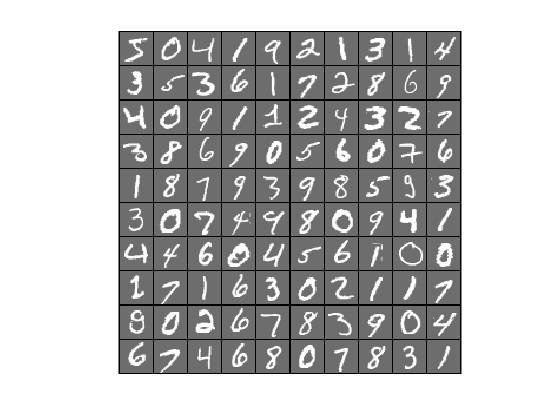
\includegraphics[width=0.9\columnwidth]{pic11.jpg}
% \caption{Dataset Description}
% \label{Dataset Description}
% \end {figure}

% describe the workloads and the ranges for each parameter you tune
The workload can be divided into two parts. First we implement the Convolutional Neural Network by hand. This includes the construction of the convolution layer, pooling layer, fully-connected layer, and the output layer.


By training the CNN, we estimate the parameters, which are the weights in each neuron. The workload is pretty large since we need to iteratively optimize the parameters using stochastic gradient descent. To be more specific, during the back propagation, we calculate the error term for each parameter and then update each one backwards. 

For the second part, we firstly connect all the terminals together and then try if they could communicate with each other correctly. Then we implement distribution method based on the framework in the first step.  

As for the parameters, we change the number of convolution layers in the CNN model in order to see the different performance: the accuracy and the efficiency. Theoretically, with more convolution layers, the model becomes more accuracy since it could better select the features in the images, while it also takes a much longer time to train the model.

The other factors that influences our experiment is the number of terminals that we use for distributed computing.  Firstly we test our distribution computing method in single machine, and if it works, we then apply it with 2, 4 machines to see how it performs.

% Describe the programming language of your implementation

For the Convolutional Neural Network, we use Python to implement this model. To be more specific, we use the Tensorflow library to better construct the CNN model. For the distributed computing we also use Python to write the framework to do the distribution.
% Describe the hardware and operating system used to run the experiments

We have 4 terminals in total that were used in the experiment. We don't use them all in every experiment, and the number varies based on the requirement. The description of operating system and hardware is as follows:

Terminal 1 (main): Windows 8.1, 64-bit operating system based on 64x CPU; Intel Core i5-4210U, 1.70 GHz CPU; and 6.00 GB RAM.  Terminal 2: Windows 8.1, 64-bit operating system based on 64x CPU; Intel Core i5-4405U, 2.10 GHz CPU; and 6.00 GB RAM.  Terminal 3: Windows 8.1, 64-bit operating system based on 64x CPU; Intel Core i7-6700HQ, 3.50 GHz CPU; and 8.00 GB RAM.  Terminal 4: Windows 8.1, 64-bit operating system based on 64x CPU; Intel Core i5-6200U, 2.80 GHz CPU; and 6.00 GB RAM.


\subsection{Experiment 1}
\label{subsec:Exp1}

In the first experiment, we use naive CNN model to verify how the neural network performs when dealing with the handwritten digit recognition with or without the elastic distortion. In order to make reasonable comparison, we used both normal and elastic data set, and also different number of layers in the model. Fig. ~\ref{Case study error rate based on different layers and different input data} shows the accuracy results in different cases:

\begin {figure}[t]
\centering
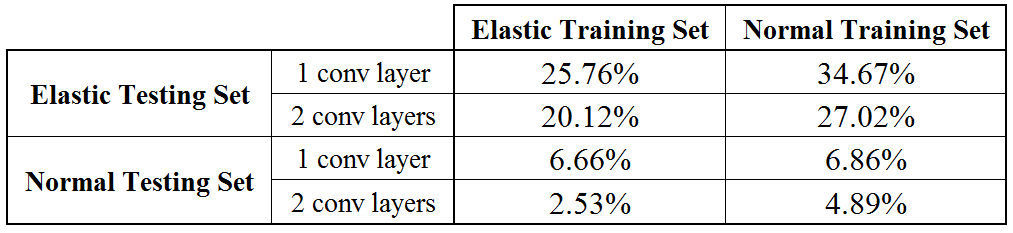
\includegraphics[width=0.90\columnwidth]{ResultsTbl1.png} % pic17.png
\caption{Case study error rate based on different layers and different input data.}
\label{Case study error rate based on different layers and different input data}
%\vspace{-10pt}
\end {figure}



\subsubsection*{Case 1: Normal Training vs Elastic Training} 

First we used the CNN with one convolution layers and use normal testing data set. In this case
we want to see if the elastic distortion would improve the accuracy, thus we compared the elastic training data and normal training data. From the third row of Fig. ~\ref{Case study error rate based on different layers and different input data}, we could see that the elastic training set could slightly improve the accuracy.

Now we want to use two convolution layers. In the last row of Fig. ~\ref{Case study error rate based on different layers and different input data}, we can see two facts: 1) the one more convolution layer can improve accuracy in both training data sets; 2) The influence from the elastic distortion is bigger when there are two convolution layers than one.

\begin {figure}[t]
\centering
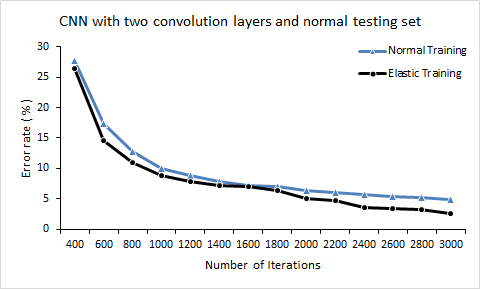
\includegraphics[width=0.9\columnwidth]{Paper_Fig7_Conv_Case1.png} % pic20.jpg
\caption{Convergence for Normal Training VS Elastic Training.}
\label{Convergence plot in case 1}
\end {figure}



We also want to know the convergence rate when using normal training data set and elastic training data set. As we can see from Fig. ~\ref{Convergence plot in case 1}, these two training data sets mainly gives the same convergence rate, and the accuracy is stable after about 2000 iterations.

\subsubsection*{Case 2: Elastic Testing Data}

In order to make the problem more challenging, we then used to model to test the elastic testing data set. 

\begin {figure}[t]
\centering
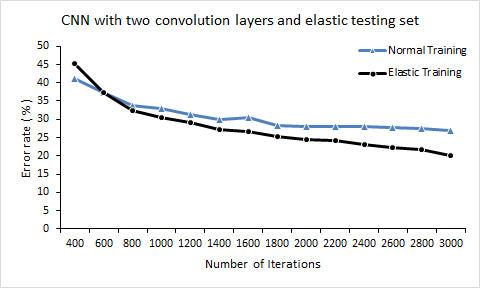
\includegraphics[width=0.9\columnwidth]{Paper_Fig8_Conv_Case2.png} % pic21.jpg
\caption{Convergence for Elastic Testing Data.}
\label{Convergence plot in case 2}
\vspace{-10pt}
\end {figure}


The plot above is when we used elastic testing data set and two convolution layers. We can see that the elastic training data set in this case also gives better performance than normal training data set. In addition, the error rate in Fig. \ref{Convergence plot in case 2} is much larger than that in Fig. \ref{Convergence plot in case 1}. The reason is that the distortion in testing case badly influenced the recognition, which made the whole accuracy decrease. They became stable almost at the 3000 iterations.

\subsubsection*{Case 3: Noisy Testing Data}

Now we want to see if the elastic distortion technique could partially or totally solve the problem with noisy testing data. So we add some salt and pepper noise in the testing data set.

\begin {figure}[t]
\centering
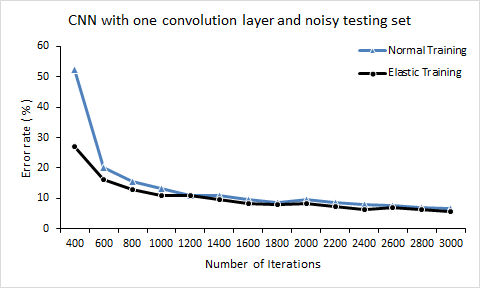
\includegraphics[width=0.9\columnwidth]{Paper_Fig9_Conv_Case3.png} % pic22.jpg
\caption{Convergence for Noisy Testing Data.}
\label{Convergence plot in case 3}
\end {figure}


From Fig. ~\ref{Convergence plot in case 3} we can see that, with elastic distortion, the CNN can deal with the noise better than
normal testing data set. For the convergence rate, they are both stable after about 1500 iterations.

\subsubsection*{Case 4: Convolution Layers}

In this case we compared the results when using different number of convolution layers.

\begin {figure}[t]
\centering
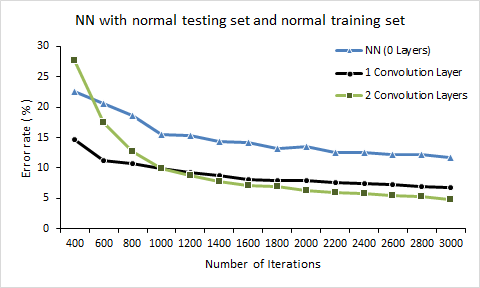
\includegraphics[width=0.9\columnwidth]{Paper_Fig10_Conv_Case4.png} % pic23.jpg
\caption{Convergence for Convolution Layers.}
\label{Convergence plot in case 4}
\vspace{-10pt}
\end {figure}


The line with triangle markers in Fig. \ref{Convergence plot in case 4} is the model with 0 convolution layer, which is just the normal neural network (NN). The line with circle markers is the model with 1 convolution layer (CNN-1L) and the line with square markers is the model with 2 convolution layers (CNN-2L). From the large gap between the endpoints of the lines representing NN (triangle) and CNN-1L (circle), we can see the convolution layer actually improved accuracy. However, the endpoints of the lines representing CNN-1L (circle) and CNN-2L (square) are very close, which means the accuracy gained is relatively smaller from 1 convolution layer to 2 convolution layers. They converged to the final values after about 2000 iterations. Still, using 2 convolution layers resulted in the lowest error rate. 

\begin {figure}[t]
\centering
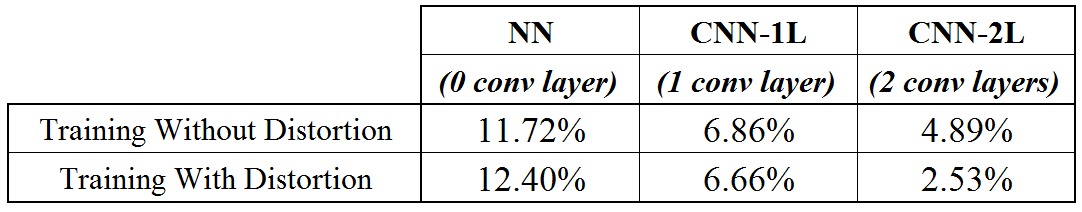
\includegraphics[width=0.90\columnwidth]{ResultsTbl2.png} % pic19.png
\caption{Error rate comparison between elastic training dataset and non-elastic training dataset.}
\label{Error rate comparison elastic and non-elastic}
\end {figure}


It is clear by looking at Fig. \ref{Error rate comparison elastic and non-elastic} that the elastic distortion works best when using 2 convolution layers (from the last column), and works second best when using 1 convolution layer (from the second-to-last column).

This trend of improvement shows that the convolution process is able to capture the local feature of each part, including the distortion, while the neural network doesn’t have this advantage.

\subsection{Experiment 2}
\label{subsec:Exp2}

In experiment we did case study about how the CNN model performs. Now we want to see if our distributed computing could indeed improve the efficiency.

\subsubsection*{Case 1: pseudo distributed computing}

Firstly we try to implement the pseudo distributed computing on single machine, this step is to verify that our implementation is correct, which results in two processes simultaneously work to do the training process. Fig. \ref{CPU utilization in case 1} shows the CPU utilization of the two processes on single machine. Since our computation is CPU-based, the CPU utilization is a reasonable measurement to check if these two processes work for our distributed CNN model. Since the machine used here is 4 cores CPU, we can see that the working utilization is near 200\% for each process, which means each one takes use of 2 cores.


\begin {figure}[t]
\centering
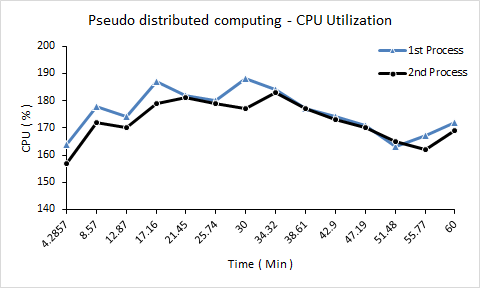
\includegraphics[width=0.9\columnwidth]{Paper_Fig12_CPU_Case1.png} % pic24.png
\caption{CPU utilization for Normal Training vs Elastic Training.}
\label{CPU utilization in case 1}
\end {figure}

\subsubsection*{Case 2: two terminals distributed computing}

Now we use two machines to do the parallel computing for the training process. Fig. \ref{CPU utilization in case 2} shows the CPU utilization in this case. We can see that, with each training process in one machine, that process is able to take use of 4 cores in one machine, which means the computation cost would be reduced.

\begin {figure}[t]
\centering
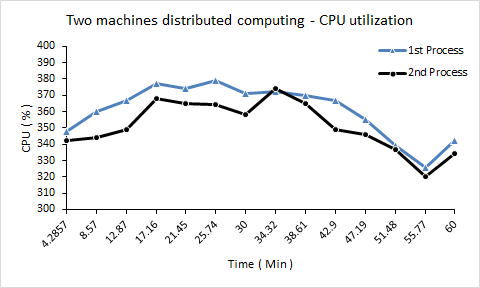
\includegraphics[width=0.9\columnwidth]{Paper_Fig13_CPU_Case2.png} % pic25.png
\caption{CPU utilization for Elastic Testing Data.}
\label{CPU utilization in case 2}
\end {figure}

\subsubsection*{Case 1: 4 terminals distributed computing}

Now we try all the 4 machines to do the distributed computing. Fig. ~\ref{CPU utilization in case 3} shows that all the processes work simultaneously to do the training process.

\begin {figure}[t]
\centering
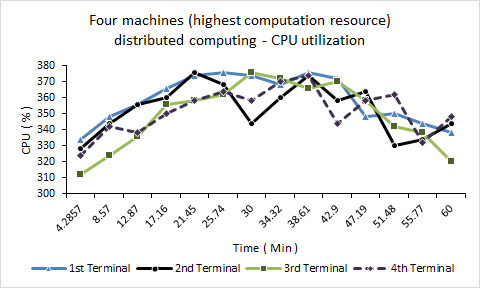
\includegraphics[width=0.9\columnwidth]{Paper_Fig13_CPU_Case3.png} % pic26.png
\caption{CPU utilization for Noisy Testing Data.}
\label{CPU utilization in case 3}
\end {figure}

Besides the cases above, we also change the number of training data in the training process to see the trend of the time consumption.

Fig. ~\ref{Execution time with different distribution methods} shows the execution time with different distributed computing method. The x-axis indicated the time consumption, and the y-axis indicates the number of training data used in the training process.

There are six bars in each of the four cases with different number of training data. The bars with vertical lines at the bottom in each group indicate the pseudo distribute method, the bars with dots in the middle indicate the 2-terminal distributed method, and the bars with the diagonal lines at the top indicate 4-terminal distributed method. Moreover, we use the dark (shaded) bar in each pattern to indicate the practical time cost and the light (non-shaded) bar in each pattern to indicate the theoretical time cost.

With the plot we can see that no matter how many samples we used in the training process, the execution time cannot reach the ideal situation. This extra cost is due to the data communication between terminals, and since our network does not has an extremely fast data communication ability, this would indeed be a problem that undermines the efficiency improvement.


\begin {figure}[t]
\centering
% Was: pic27.jpg
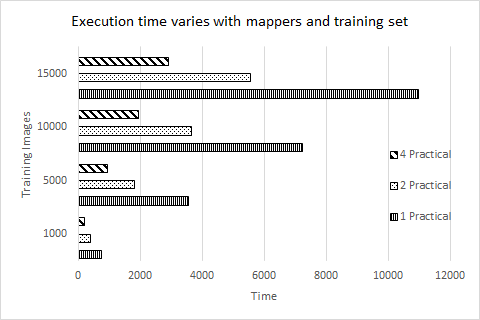
\includegraphics[width=1\columnwidth]{FigExecutionTime.png}
\vspace{-10pt}
\caption{Execution time with different distribution methods}
\label{Execution time with different distribution methods}
\vspace{-10pt}
\end {figure}

Fig. \ref{Accuracy with different distribution methods} shows the accuracy performance when we used one or two or four machines after training different number of inputs. In one hand, test accuracy climbs when more training data was involved. It follows the obvious machine learning rule, more training data covering more situations, more precious the model can represent the characteristics of this dataset. The vertical axis indicates accuracy rate while the horizon axis shows how many image used before we got that model. One the other hand, we want to see if using distribution system would have an effect on result performance. Turns out whatever the number of co-work machines, the final results don't change at all. One or two or four machine working at the same time. This figure proves that distribution computation does not change the final result for CNN training problem. 

\begin {figure}[t]
\centering
% Was pic28.jpg
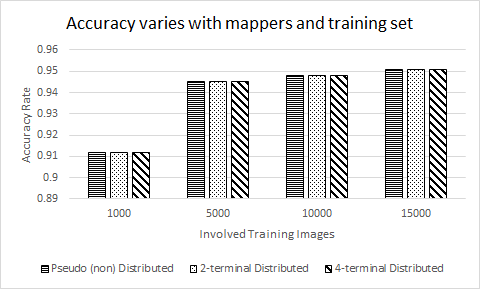
\includegraphics[width=1\columnwidth]{FigAccuracyPerf.png}
\vspace{-10pt}
\caption{Accuracy with different distribution methods}
\label{Accuracy with different distribution methods}
\vspace{-10pt}
\end {figure}


\subsection{Experimental Summary}
\label{subsec:ExpSummary}

In summary, we have shown that implementing a distributed model doesn't affect the accuracy of the results - that is, moving from a non-distributed model to a distributed one doesn't negatively impact the accuracy of the result (see Fig. \ref{Execution time with different distribution methods}) It is also clear from this same figure (Fig. \ref{Execution time with different distribution methods}) that the more distributed the model, the faster execution time becomes. Going from the non-distributed method to the 2-terminal distributed method execution time is reduced by about 50\%; execution time is reduced by a further 50\% going from the 2-terminal distribution method to the 4-terminal distributed method.  

Our results yield favorable error rates when utilizing two convolution layers and elastic training (with distortion). Fig. \ref{Error rate comparison elastic and non-elastic} shows that the error rate drops by about 10\% when training with distortion and moving from 0 convolution layers (NN) to 2 convolution layers (CNN-2L) (See bottom row of Fig. \ref{Error rate comparison elastic and non-elastic}). Even when non-elastic training was used, the error rate drops by about 7\% when moving from 0 convolution layers (NN) to 2 convolution layers (CNN-2L). In both cases it is clear the accuracy is improved when increasing from 1 convolution layer (CNN-1L) to 2 convolution layers (CNN-2L). 

The results in Fig. \ref{Error rate comparison elastic and non-elastic} are also reflected in Fig. \ref{Case study error rate based on different layers and different input data} along with error rates when elastic testing was used. With elastic training and normal testing with 2 convolution layers we achieve the lowest error rate (2.53\%). This error rate is an improvement upon the case with normal training and normal testing with 2 convolution layers (4.89\%). The effectiveness of these experiments using 1 convolution layer did not differ much between elastic and normal training sets, but were worse than the error rates using 2 convolution layers (6.66\% instead of 2.53\% error rate for elastic training, going from 1 convolution layer to 2 convolution layers; and 6.86\% instead of 4.89\% error rate for normal training set, going from 1 convolution layer to 2 convolution layers.) Generally the error rates were worse when using elastic testing set due to the increased complexity. Still we achieve about 7\% improvement when using 2 convolution layers: from 27.02\% error rate using normal training set and elastic testing set to 20.12\% error rate using elastic training set and elastic testing set. As expected, he results using elastic training are even worse when using 1 convolution layer: 25.76\% using elastic training set and 34.67\% using normal training set. 




% ======= END OF SECTION =======